\section{Data Science}
Eduard Groeller

The progressing digitalization of all aspects of human activities has tremendously increased the available data and their complexity with respect to volume, veracity, velocity, and variety. Terms like big and smart data have been coined to point towards a fourth way of scientific knowledge generation. Following experimental sciences, theoretical sciences and computational sciences, the rather new field of data science has been rapidly emerging in recent years. Data science extracts knowledge from data in a generalizable way. It explores, abstracts, and communicates intricate systems through simplified models derived from data. Based on large and rapidly growing data repositories, artificial intelligence, machine and deep learning, with subareas like convolutional neural networks (CNN), have exploded in scientific research and public attention. The academic educational system is only beginning to adjust their curricula to the appertaining challenges. A rapid increase in the analytics and data science job market is predicted, where the data scientists will have to master a very diverse skill set. Examples include the use of programmable tools to prepare and preprocess the data, generating engaging visualizations, estimating the confidence of the generated results, and automating the analysis process to increase repeatability. Learning data science involves very many miscellaneous fields like: mathematical and computer science foundations, statistics, programming, artificial intelligence and machine learning, text mining with natural language processing, visualization, big and smart data mining and management, data ingestion and wrangling, applying and integrated use of various toolboxes. Computer science is a key basis and enabling technology in many of these subareas. The rapid evolution of the field of data science and its inherent very large diversity concerning technological approaches and application areas, make the specification, shaping, and localization of data science curricula especially challenging.

\subsection{Data Science's Home Department}

Data Science is located in about 46\% of cases at the informatics departments (see Figure~\ref{sect4:discipline}). In 30\% of the cases data science is jointly handled by the informatics and mathematics/statistics departments. Even more than two departments are jointly organizing data science activities in 13\% of the cases. Only in 7\% of the cases a single department other than computer science (e.g., statistics, economics, mathematics) is the main responsible unit. This distribution indicates the central role of computer science in the developing field of data science. Data science is happening in almost all disciplines, but the highest concentration of expertise and courses seem to be in the computer science and statistics departments. Sometimes data science and artificial intelligence are seen as cross-sectional disciplines, which are governed by groups of interested departments (from mathematics and logic to sociology and philosophy). The Utrecht University is an example in this respect. The economic and business departments were also mentioned several times as participating together with computer science and mathematics in data science activities. Examples of other single department set-ups have been given, like bio-nano sciences (Babes-Bolyai Universuty Cluj-Napoca), economics studies department (Universit\`a degli studi G.D’Annunzio Chieti Pescara), statistics department (University of Almeria).

\begin{figure}[h]
\centering
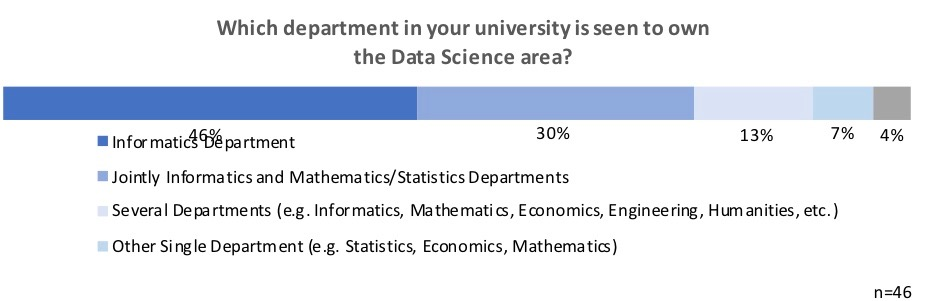
\includegraphics[width = \linewidth]{charts/4a.jpg}
\caption{Data science is part of what discipline?}
\label{sect4:discipline}
\end{figure}

\subsection{Perception of Informatics}

A large majority of 61\% of respondents indicated that the rise of data science has changed the perception of informatics in the respective university (see Figure~\ref{sect4:}). Ethics and other social science aspects are considered to be increasing in relevance. There are initiatives to develop introductory courses on digital literacy and skills in all study programs (e.g., at Delft University of Technology, TU Wien). The importance of information technology is considered to be increasing beyond computational thinking to cover topics like data science and machine learning. Computer science is considered to be the main knowledge center in the digital transformation of society and many initiatives are under way that are changing how informatics is perceived. A growing number of non-informatics departments are asking informatics departments to teach data science courses. Also, a tendency towards interdisciplinary curricula is observable (like a bridge to statistics and economics). At many places computer science is recognized as an integrated part of the transformative processes currently underway. The increased relevance of informatics is reflected in higher funding and a surge of interest in data science studies by potential (computer science) students.

\begin{figure}[h]
\centering
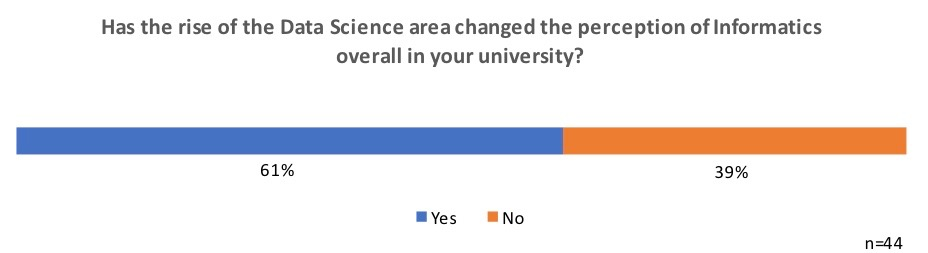
\includegraphics[width = \linewidth]{charts/4b.jpg}
\caption{Has the perception of Informatics changed with the rise of Data Science?}
\label{sect4:}
\end{figure}

\subsection{Current Arrangements at Universities}

The initiative on digital skills programs coming from the top university level beyond the computer science department might be positive in supporting implementation acceptance (Delft University of Technology). At other places the university upper levels consider the scientific and societal impact of data science and artificial intelligence rather in the (external) application domains, although an increase in informatics students is recognizable. The early awareness of data science and machine learning as areas of rapidly increasing importance is considered crucial. Due to inertial forces (especially at larger universities), however, sometimes active strategies from the top university level is lagging, though bottom up approaches might compensate for this. As in analogous situations in the past, informatics is struggling to be viewed only as a service department to help other domains in solving their data science problems. This is similar to previous interdisciplinary approaches (e.g., multimedia, computer graphics, animation) where informatics is used as a tool, but gradually also as a research partner on an equal footing. The surge in interest in data science is accompanied by larger resource flows. The uncertainty about where to locate the data science activities might lead to the simultaneous development of several research groups at one university. This decentralized approach might allow the different departments to grow and manage their own data science groups with discriminative strengths. The quickly amplified interest in data science is primarily considered an opportunity, where it is challenging to follow and sustain all parallel activities. Currently the interest in data science, machine learning, and artificial intelligence is so large that this might overshadow all other areas of computer science and informatics. Too imbalanced funding opportunities and student flows should be avoided to provide a well-adjusted portfolio of competences to the society and economy.

\subsection{Final Thoughts}

The interest and popularity of data science and artificial intelligence has dramatically risen in the last 10-20 years. These technologies have the potential to be driving and enabling technologies for the rapidly unfolding digital transformation of society. The very fast developments lead to many daunting challenges, e.g., concerning privacy, security, bias, reliability, robustness, legal and ethical implications. It is not yet clear where data science should be anchored, e.g., in the computer science department, multi-department units, application domains, aso. Due to the developmental speed, established organizations like universities are struggling to swiftly adjust their organizational structures and educational portfolios, where long term changes have yet to be implemented. For some experts in potential applications fields data science and artificial intelligence might be perceived as a hype that will cool down eventually. Despite this, most experts see the pervasive utility of computer science tools for their research area. The data scientist as a profession will be much more heterogeneous in the required skill set as compared to other interdisciplinary approaches, like business informatics, bio-informatics, or medical informatics, which basically involve two disciplines each. Considering the wide array of concerned fields, the data scientist will have a deep knowledge in just one or a few specialties and have a broad (and shallow) knowledge of the many other concerned areas. Data science encompasses a mixture of multidisciplinary skills ranging from mathematics/statistics, programming/databases, domain knowledge/soft skills, communication and visualization. The fluidity of the development and the breadth of the area will transfer to data science groups, centers, and curricula with largely varying specializations. It seems very likely that computer science will play a key role in all these developments, where we should pro-actively use the many emerging opportunities.
